\documentclass[a4paper, 11pt]{article}

% Nécessaire
\usepackage[french]{babel}
\usepackage[utf8]{inputenc}
\usepackage[T1]{fontenc}
\usepackage{lmodern}
\usepackage{amsmath, amsthm}
\usepackage{amsfonts,amssymb}

% Marge
\usepackage{geometry}
\geometry{margin={2.2cm ,2cm}}

% Figures, graphiques
\usepackage{graphicx}
\usepackage{epsfig}
\usepackage{caption}

% Surlignage
\usepackage{alltt}

\usepackage{xcolor}
\usepackage{soul}
\usepackage{color}
\usepackage{colortbl}

% Indicatrice
\usepackage{dsfont}

\usepackage{multirow}
\usepackage{eurosym}
\usepackage{extarrows}

% Graphique
\usepackage{tikz}


% Titre
\title{Modification des processus biologiques}
\author{}
\date{}



\begin{document}
\maketitle  

On essaye ici de modifier certaines hypothèses du modèle et voir les modifications que cela entraîne.

\section{Référence}

Les modifications effectuées seront comparées avec notre estimation de référence. Les paramètres trouvés sont :
\begin{center}
\begin{tabular}{lllll}
$\gamma$ & $p_m$ & $\mu_{ER}$ & $\mu_{EH}$ & $k$\\
0.065 & 0.798 & 0.220 & 0.000 & 43.667
\end{tabular}
\end{center}

Les dynamiques associées sont visibles sur la figure~\ref{fig:ref}.

\begin{figure}[ht]
\centering
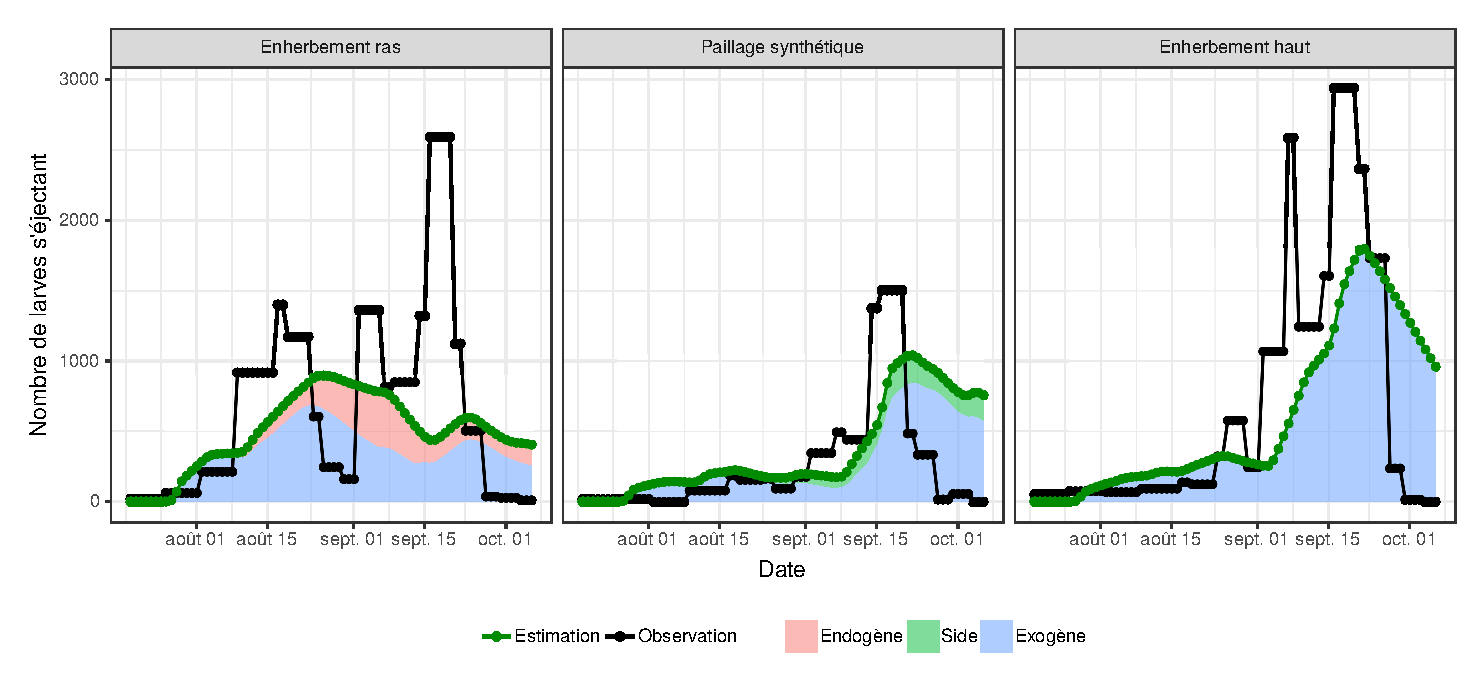
\epsfig{file = plots/proc_ref.eps, scale = 0.65}
\caption{Dynamiques de référence.}
\label{fig:ref}
\end{figure}

\newpage
\paragraph{Modification 1} Les individus exogènes n'arrivent plus proportionellement aux inflorescences. Il y a une arrivée constante de 20 individus par jour.
Les paramètres sont
{%
\newcommand{\mc}[3]{\multicolumn{#1}{#2}{#3}}
\begin{center}
\begin{tabular}{lllll}
\mc{5}{c}{Référence}\\
$\gamma$ & $p_m$ & $\mu_{ER}$ & $\mu_{EH}$ & $k$\\
0.065 & 0.798 & 0.220 & 0.000 & 43.667\\
\mc{5}{c}{Modification}\\
$\gamma$ & $p_m$ & $\mu_{ER}$ & $\mu_{EH}$ & $k$\\
/ & 0.557 & 0.556 & 0.700 & 27.52
\end{tabular}
\end{center}
}%



Résultats visibles sur la figure~\ref{fig:exo}.

\begin{figure}[ht]
\centering
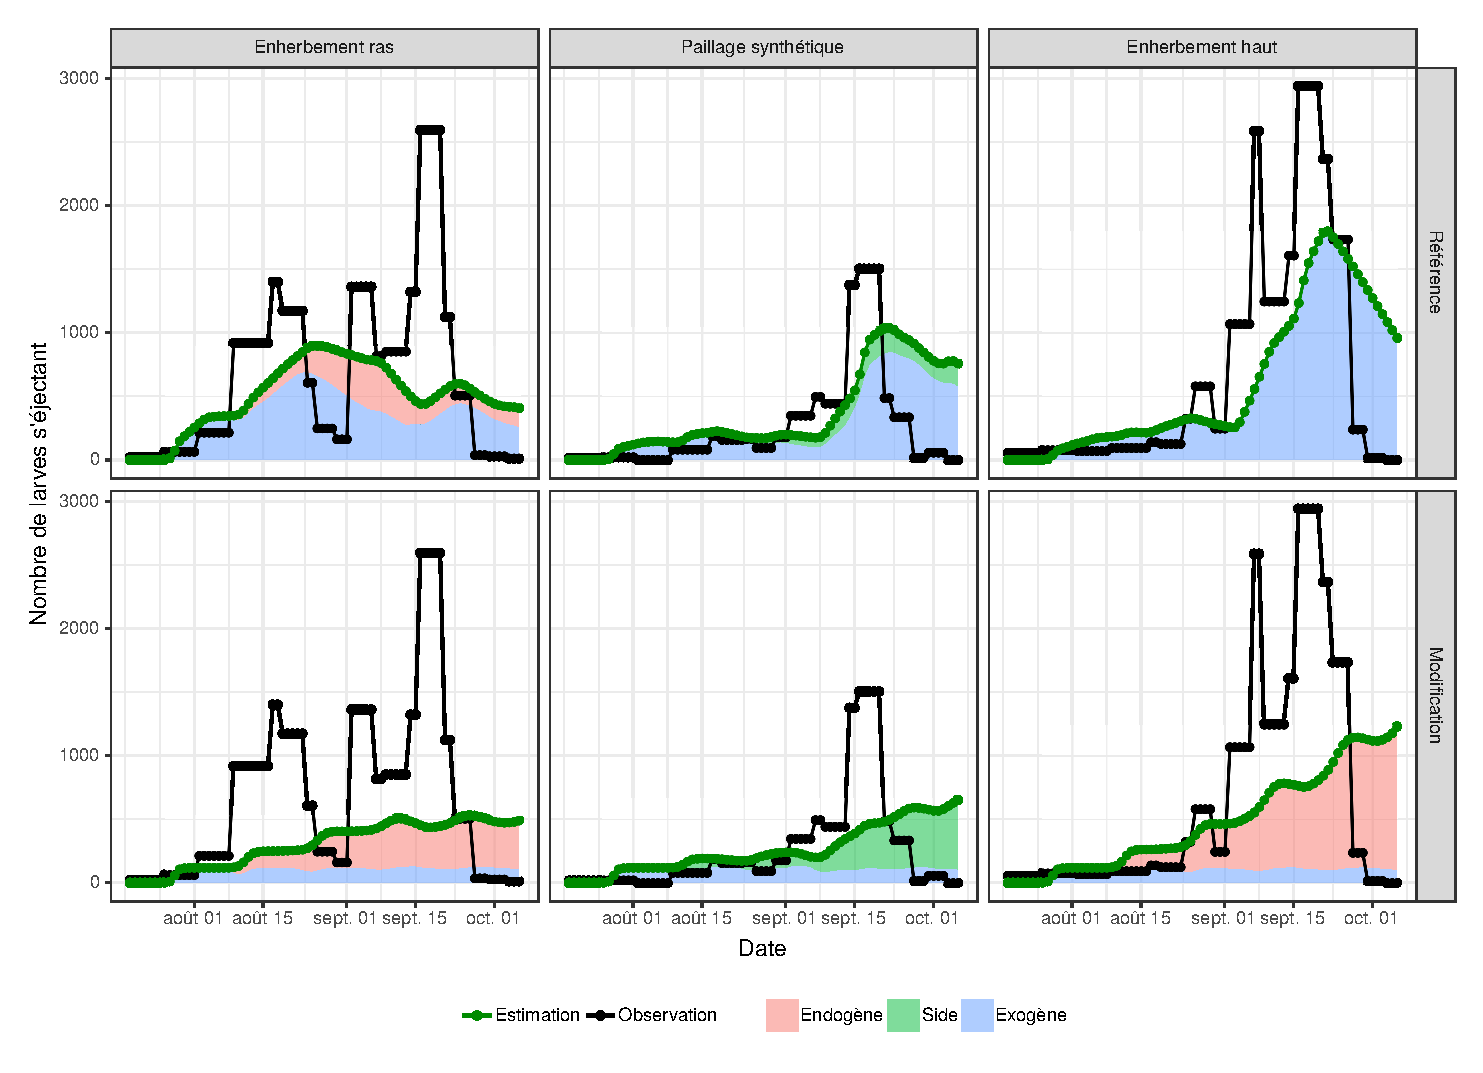
\epsfig{file = plots/proc_exogene.eps, scale = 0.65}
\caption{Comparaison référence / modification 1.}
\label{fig:exo}
\end{figure}




\newpage
\paragraph{Modification 2} Les individus émergents dans le bloc se répartisssent dans les trois sous-blocs proportionellement aux inflorescences présentes dans ces derniers.
Les paramètres sont
{%
\newcommand{\mc}[3]{\multicolumn{#1}{#2}{#3}}
\begin{center}
\begin{tabular}{lllll}
\mc{5}{c}{Référence}\\
$\gamma$ & $p_m$ & $\mu_{ER}$ & $\mu_{EH}$ & $k$\\
0.065 & 0.798 & 0.220 & 0.000 & 43.667\\
\mc{5}{c}{Modification}\\
$\gamma$ & $p_m$ & $\mu_{ER}$ & $\mu_{EH}$ & $k$\\
0.032 & / & 0.950 & 0.000 & 25.495
\end{tabular}
\end{center}
}%



Résultats visibles sur la figure~\ref{fig:exchange}.

\begin{figure}[ht]
\centering
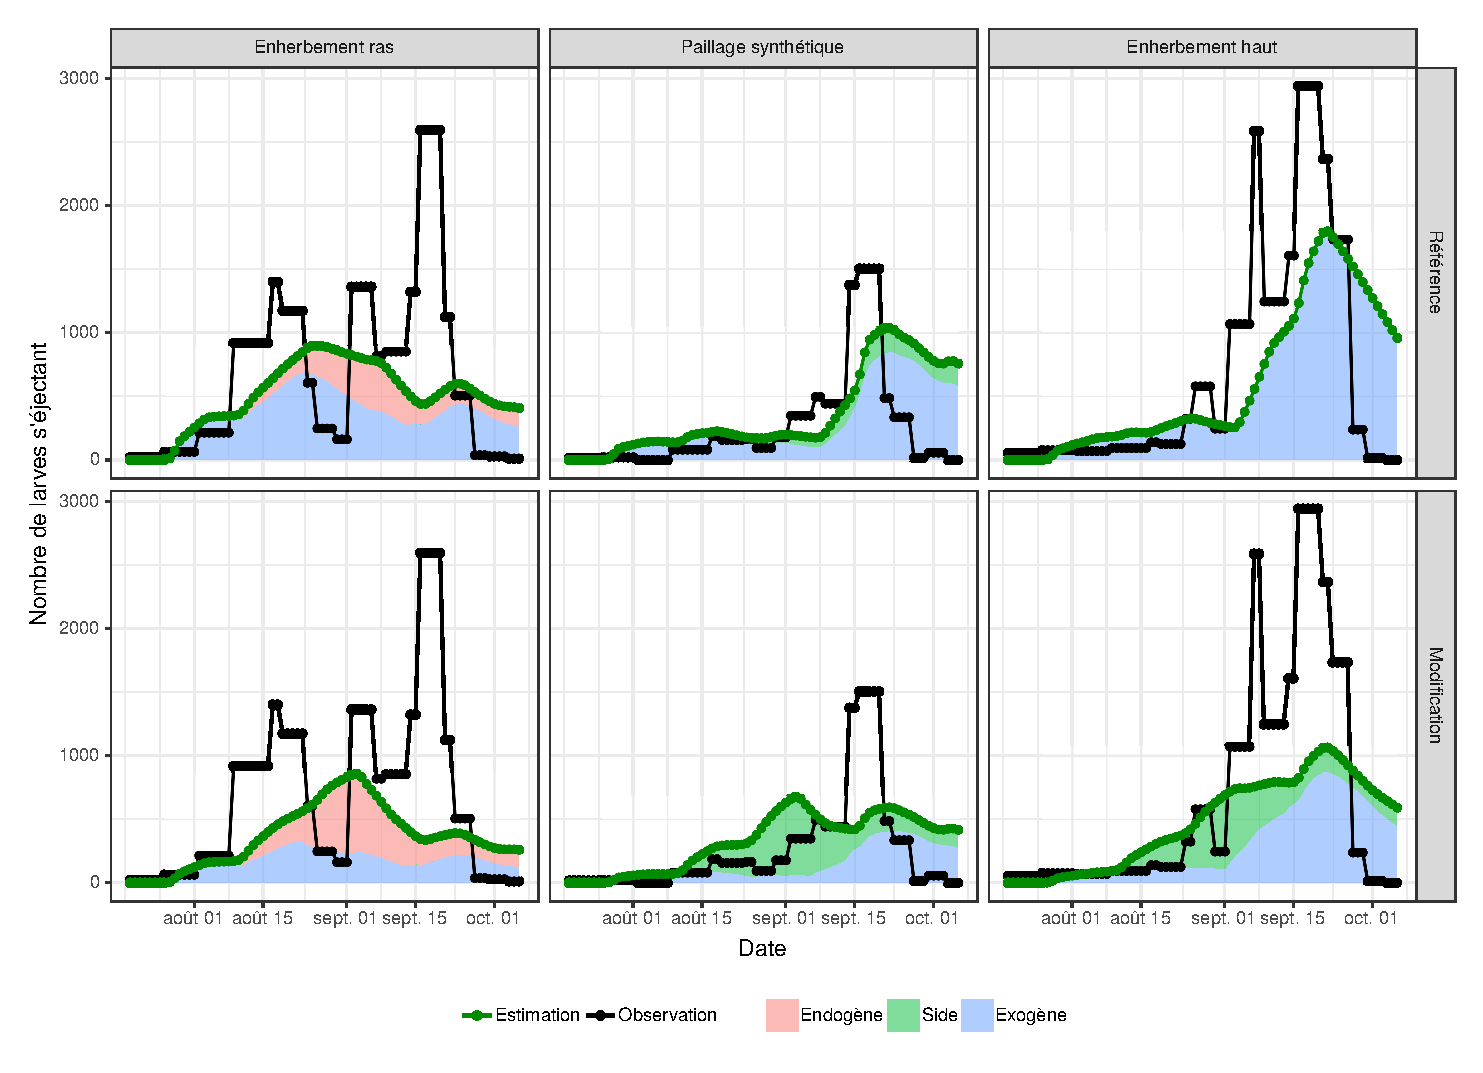
\epsfig{file = plots/proc_exchange.eps, scale = 0.65}
\caption{Comparaison référence / modification 2.}
\label{fig:exchange}
\end{figure}




\newpage
\paragraph{Modification 2 bis} Les individus émergents dans le bloc se répartisssent uniformément dans les trois sous-blocs.
Les paramètres sont
{%
\newcommand{\mc}[3]{\multicolumn{#1}{#2}{#3}}
\begin{center}
\begin{tabular}{lllll}
\mc{5}{c}{Référence}\\
$\gamma$ & $p_m$ & $\mu_{ER}$ & $\mu_{EH}$ & $k$\\
0.065 & 0.798 & 0.220 & 0.000 & 43.667\\
\mc{5}{c}{Modification}\\
$\gamma$ & $p_m$ & $\mu_{ER}$ & $\mu_{EH}$ & $k$\\
0.049 & / & 0.575 & 0.000 & 44.621
\end{tabular}
\end{center}
}%



Résultats visibles sur la figure~\ref{fig:exchangebis}.

\begin{figure}[ht]
\centering
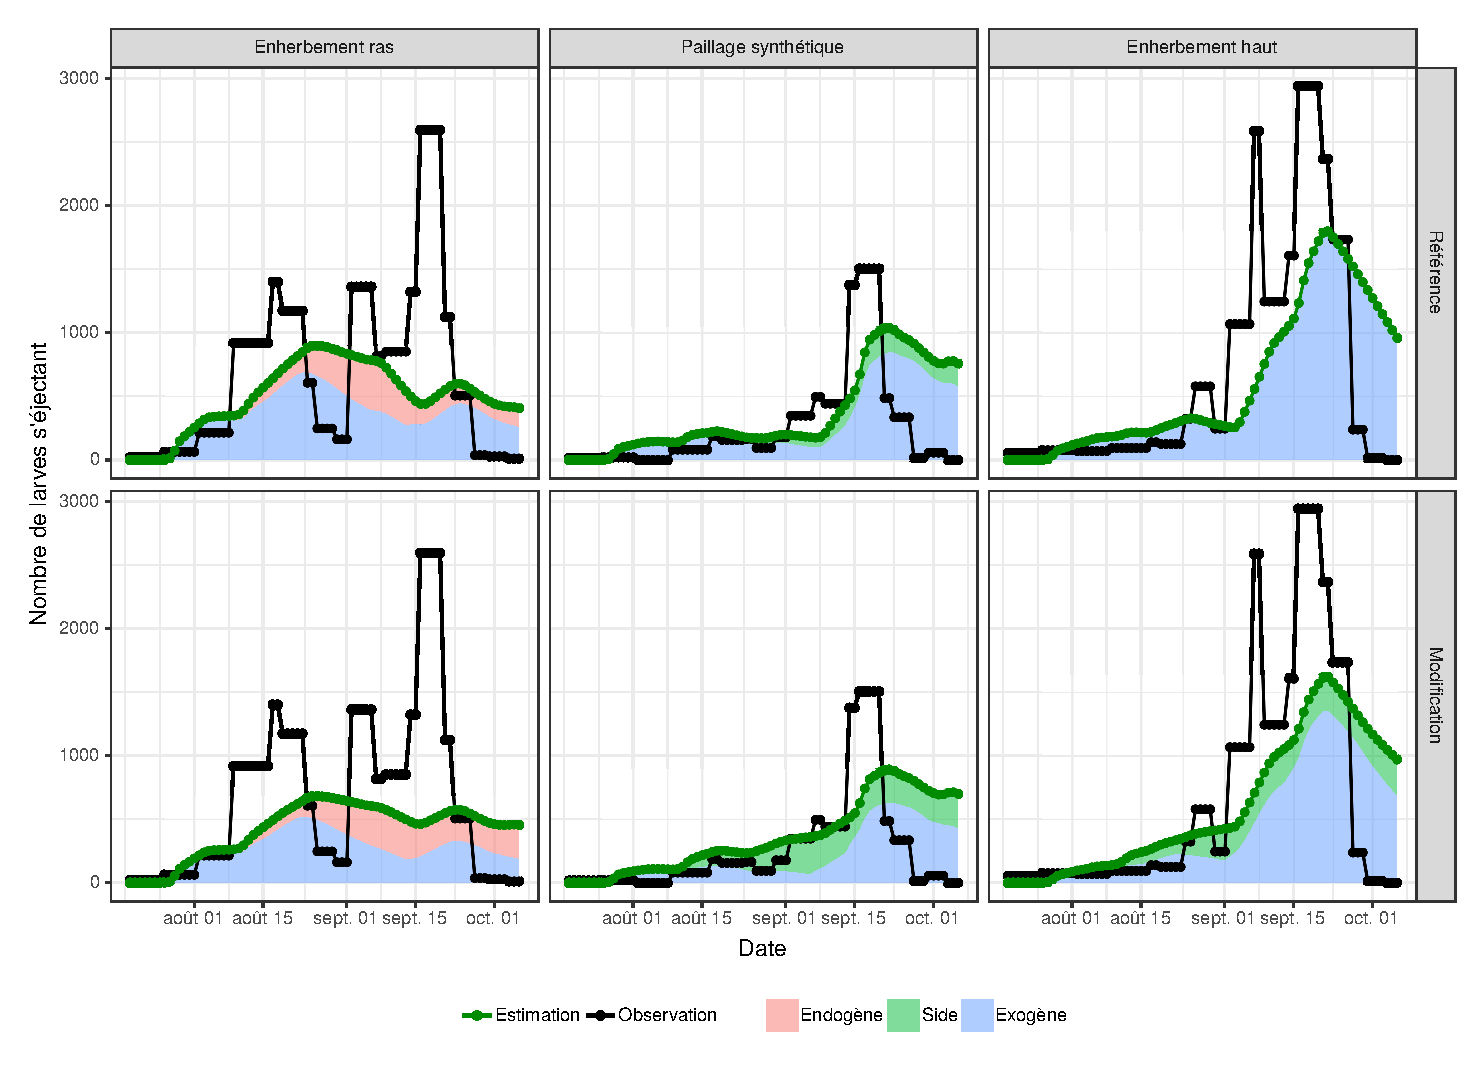
\epsfig{file = plots/proc_exchangebis.eps, scale = 0.65}
\caption{Comparaison référence / modification 2 bis.}
\label{fig:exchangebis}
\end{figure}






\newpage
\paragraph{Modification 3} Le $\mu_{global} = 2.31$ (correspondant au nombres de femelles que produit une femelle en un cycle) passe à 5. (Le nombre d'œufs pondus passe de 150 à 325).
Les paramètres sont
{%
\newcommand{\mc}[3]{\multicolumn{#1}{#2}{#3}}
\begin{center}
\begin{tabular}{lllll}
\mc{5}{c}{Référence}\\
$\gamma$ & $p_m$ & $\mu_{ER}$ & $\mu_{EH}$ & $k$\\
0.065 & 0.798 & 0.220 & 0.000 & 43.667\\
\mc{5}{c}{Modification}\\
$\gamma$ & $p_m$ & $\mu_{ER}$ & $\mu_{EH}$ & $k$\\
0.031 & 0.792 & 0.106 & 0.000 & 55.999
\end{tabular}
\end{center}
}%



Résultats visibles sur la figure~\ref{fig:eggs}.

\begin{figure}[ht]
\centering
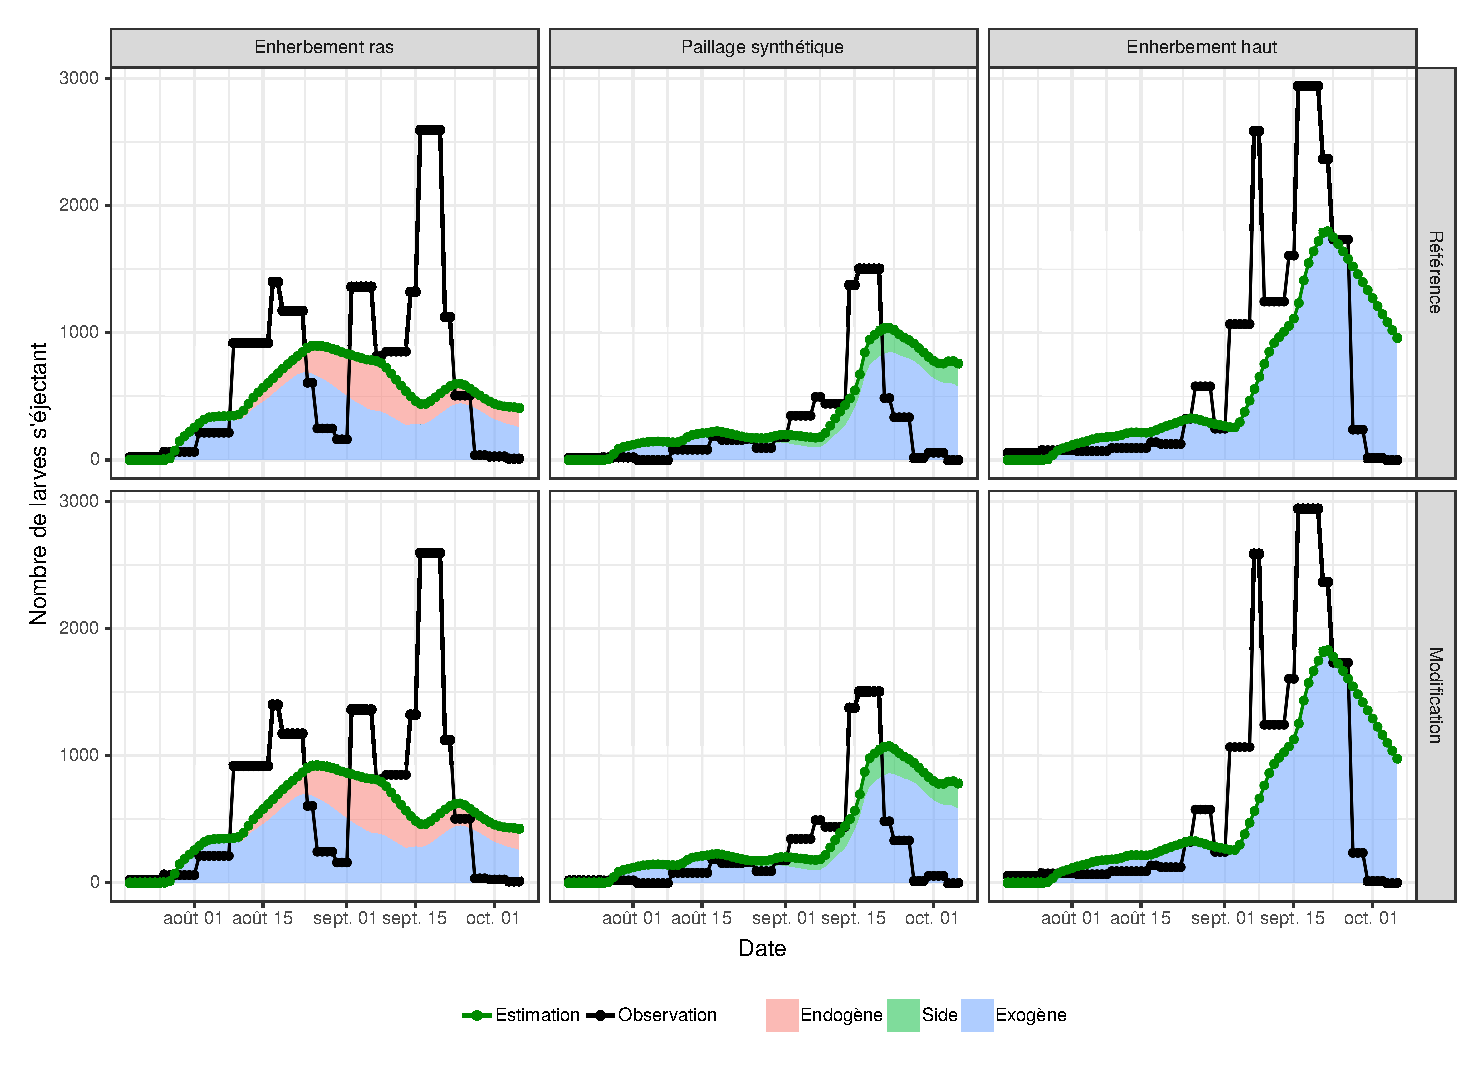
\epsfig{file = plots/proc_eggs.eps, scale = 0.65}
\caption{Comparaison référence / modification 3.}
\label{fig:eggs}
\end{figure}




\newpage
\paragraph{Modification 4} On modifie le coefficient de disponibilité en ressources pour qu'il passe de
$$
R = \min\left\{1, \frac{kI}{N}\right\} \qquad \text{à} \qquad R = \left\{1, \left( \frac{I}{N} \right)^2 \right\}.
$$
La figure~\ref{fig:calib} illustre la modification.

\begin{figure}[ht]
\centering

\begin{tikzpicture}
 \draw [very thin, lightgray, opacity = 0.5] (0,0) grid (1.9,1.9);
 \draw [->] (0, 0) -- (0, 2);
 \draw [->] (0, 0) -- (2, 0);
 \draw [domain=0:1] plot(\x, \x);
 \draw (1,1) -- (1.9, 1);
 \draw [gray] (2,0) node[right] {$I / N$};
 \draw [gray] (0,2) node[above] {$R$};
\end{tikzpicture}
\begin{tikzpicture}
 \draw [very thin, lightgray, opacity = 0.5] (0,0) grid (1.9, 1.9);
 \draw [->] (0, 0) -- (0, 2);
 \draw [->] (0, 0) -- (2, 0);
 \draw [domain=0:1] plot(\x, \x^2);
 \draw (1,1) -- (1.9, 1);
 \draw [gray] (2,0) node[right] {$I / N$};
 \draw [gray] (0,2) node[above] {$R$};
\end{tikzpicture}

\caption{À gauche (la référence), la relation entre $R$ et $I/N$ pour un $k=1$. À droite, la nouvelle relation entre $R$ et $I/N$.}
\label{fig:calib}
\end{figure}


Les paramètres sont
{%
\newcommand{\mc}[3]{\multicolumn{#1}{#2}{#3}}
\begin{center}
\begin{tabular}{lllll}
\mc{5}{c}{Référence}\\
$\gamma$ & $p_m$ & $\mu_{ER}$ & $\mu_{EH}$ & $k$\\
0.065 & 0.798 & 0.220 & 0.000 & 43.667\\
\mc{5}{c}{Modification}\\
$\gamma$ & $p_m$ & $\mu_{ER}$ & $\mu_{EH}$ & $k$\\
0.066 & 0.675 & 0.210 & 0.000 & /
\end{tabular}
\end{center}
}%



Résultats visibles sur la figure~\ref{fig:k}.

\begin{figure}[ht]
\centering
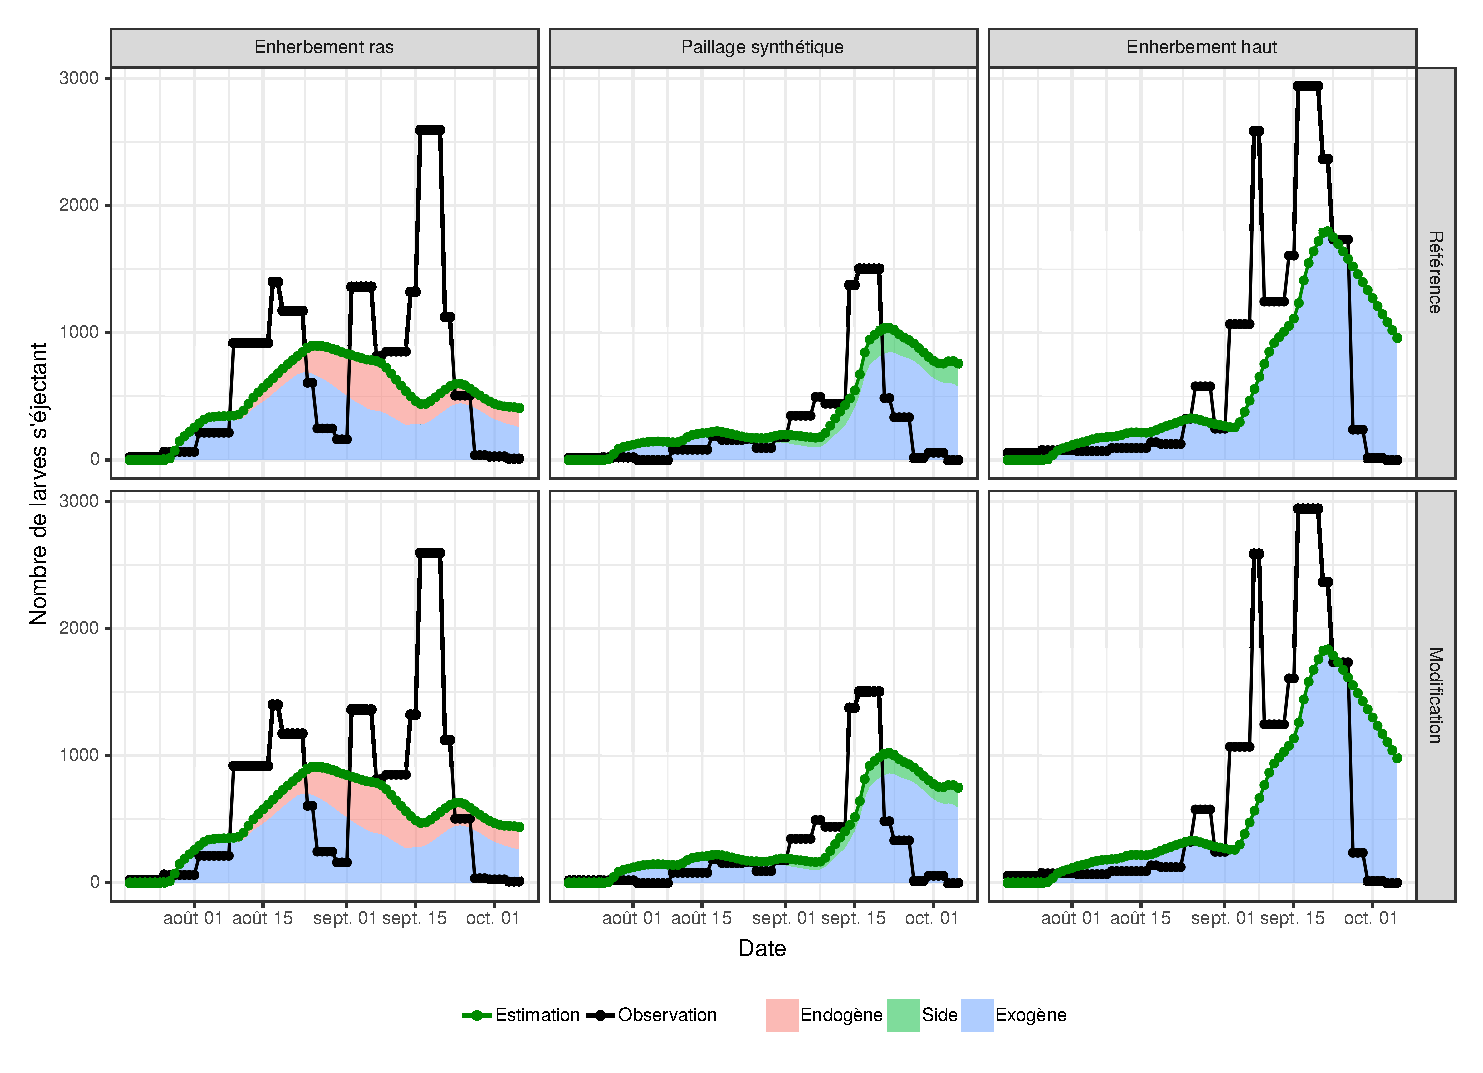
\epsfig{file = plots/proc_k.eps, scale = 0.65}
\caption{Comparaison référence / modification 4.}
\label{fig:k}
\end{figure}



\newpage
\paragraph{Modification 5} On change la fonction de coût. On ne minimise plus la fonction $MAE$ définie par
$$
MAE\left( y, \hat y \right) = \frac{1}{n}\sum_j^n |y_j - \hat y_j|,
$$
mais on essaye de minimiser l'écart maximum :
$$
f(y, \hat y) = \max_j |y_j - \hat y_j|.
$$
Les paramètres sont
{%
\newcommand{\mc}[3]{\multicolumn{#1}{#2}{#3}}
\begin{center}
\begin{tabular}{lllll}
\mc{5}{c}{Référence}\\
$\gamma$ & $p_m$ & $\mu_{ER}$ & $\mu_{EH}$ & $k$\\
0.065 & 0.798 & 0.220 & 0.000 & 43.667\\
\mc{5}{c}{Modification}\\
$\gamma$ & $p_m$ & $\mu_{ER}$ & $\mu_{EH}$ & $k$\\
0.086 & 0.029 & 0.293 & 0.026 & 51.505
\end{tabular}
\end{center}
}%



Résultats visibles sur la figure~\ref{fig:cost}.

\begin{figure}[ht]
\centering
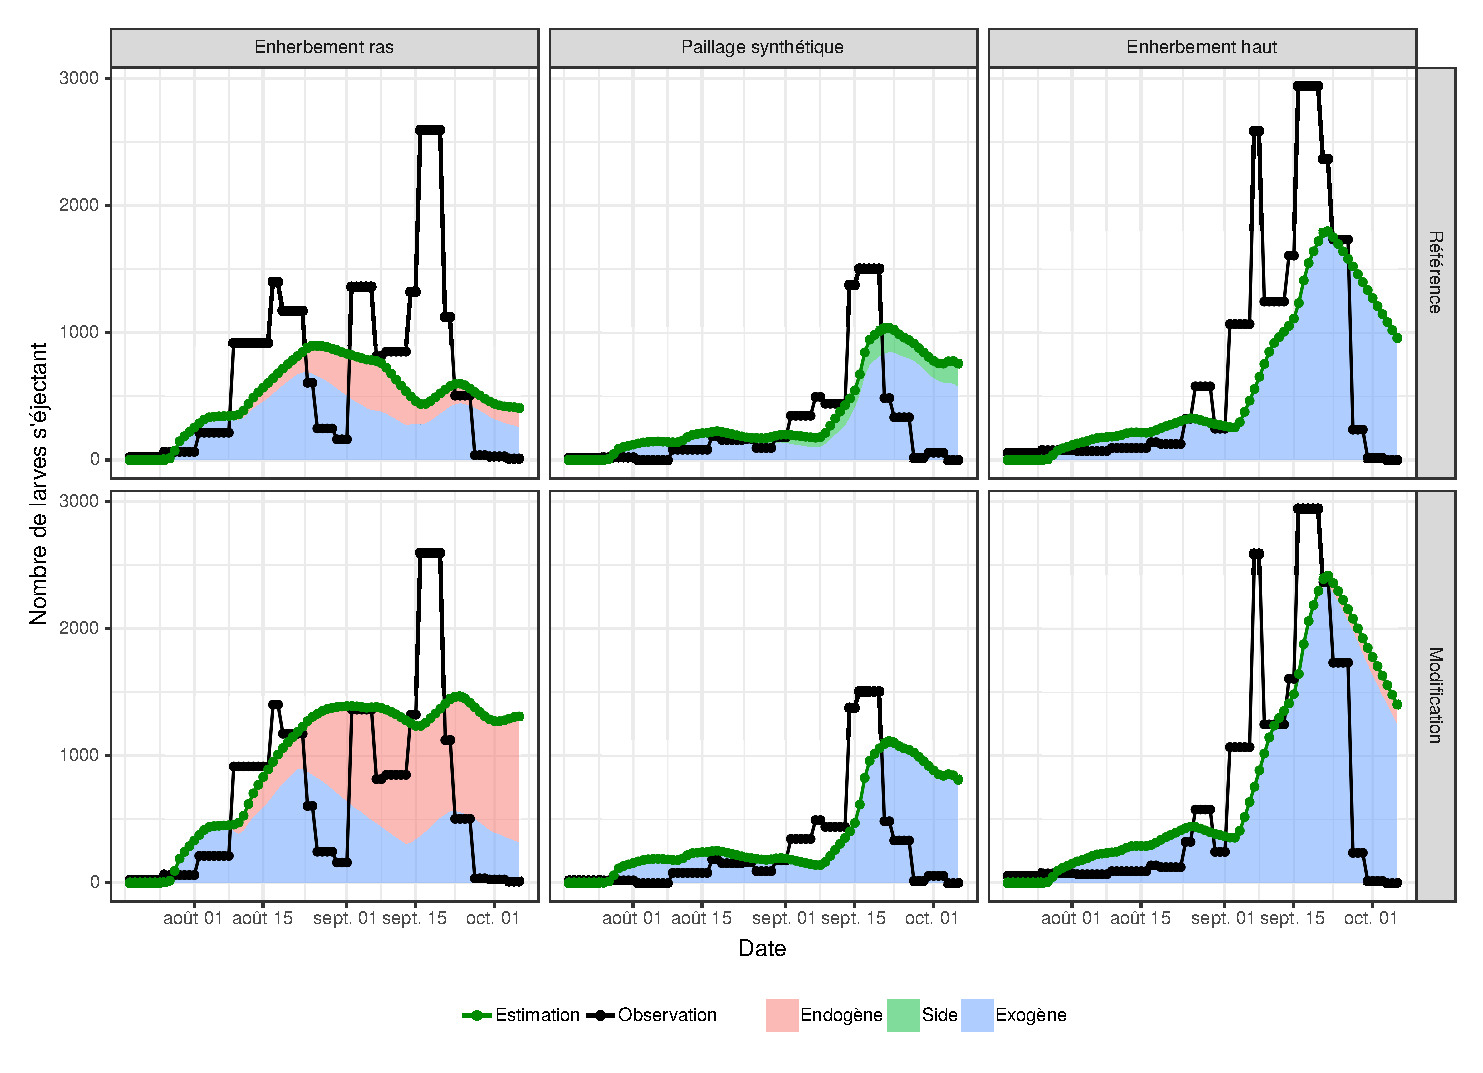
\epsfig{file = plots/proc_cost.eps, scale = 0.65}
\caption{Comparaison référence / modification 5.}
\label{fig:cost}
\end{figure}




\newpage
\paragraph{Modification 6} On introduit un paramètre de «saisonnalité» $\xi_{end}$ qui entre en jeu à partir du 15 septembre. Ce paramètre limite les femelles dans le verger à partir de cette date.
Les paramètres sont
{%
\newcommand{\mc}[3]{\multicolumn{#1}{#2}{#3}}
\begin{center}
\begin{tabular}{llllll}
\mc{6}{c}{Référence}\\
$\gamma$ & $p_m$ & $\mu_{ER}$ & $\mu_{EH}$ & $k$ & $\xi_{end}$\\
0.065 & 0.798 & 0.220 & 0.000 & 43.667 & /\\
\mc{6}{c}{Modification}\\
$\gamma$ & $p_m$ & $\mu_{ER}$ & $\mu_{EH}$ & $k$ & $\xi_{end}$\\
0.034 & 0.347 & 0.556 & 0.836 & 46.782 & 0.02
\end{tabular}
\end{center}
}%



Résultats visibles sur la figure~\ref{fig:end}.

\begin{figure}[ht]
\centering
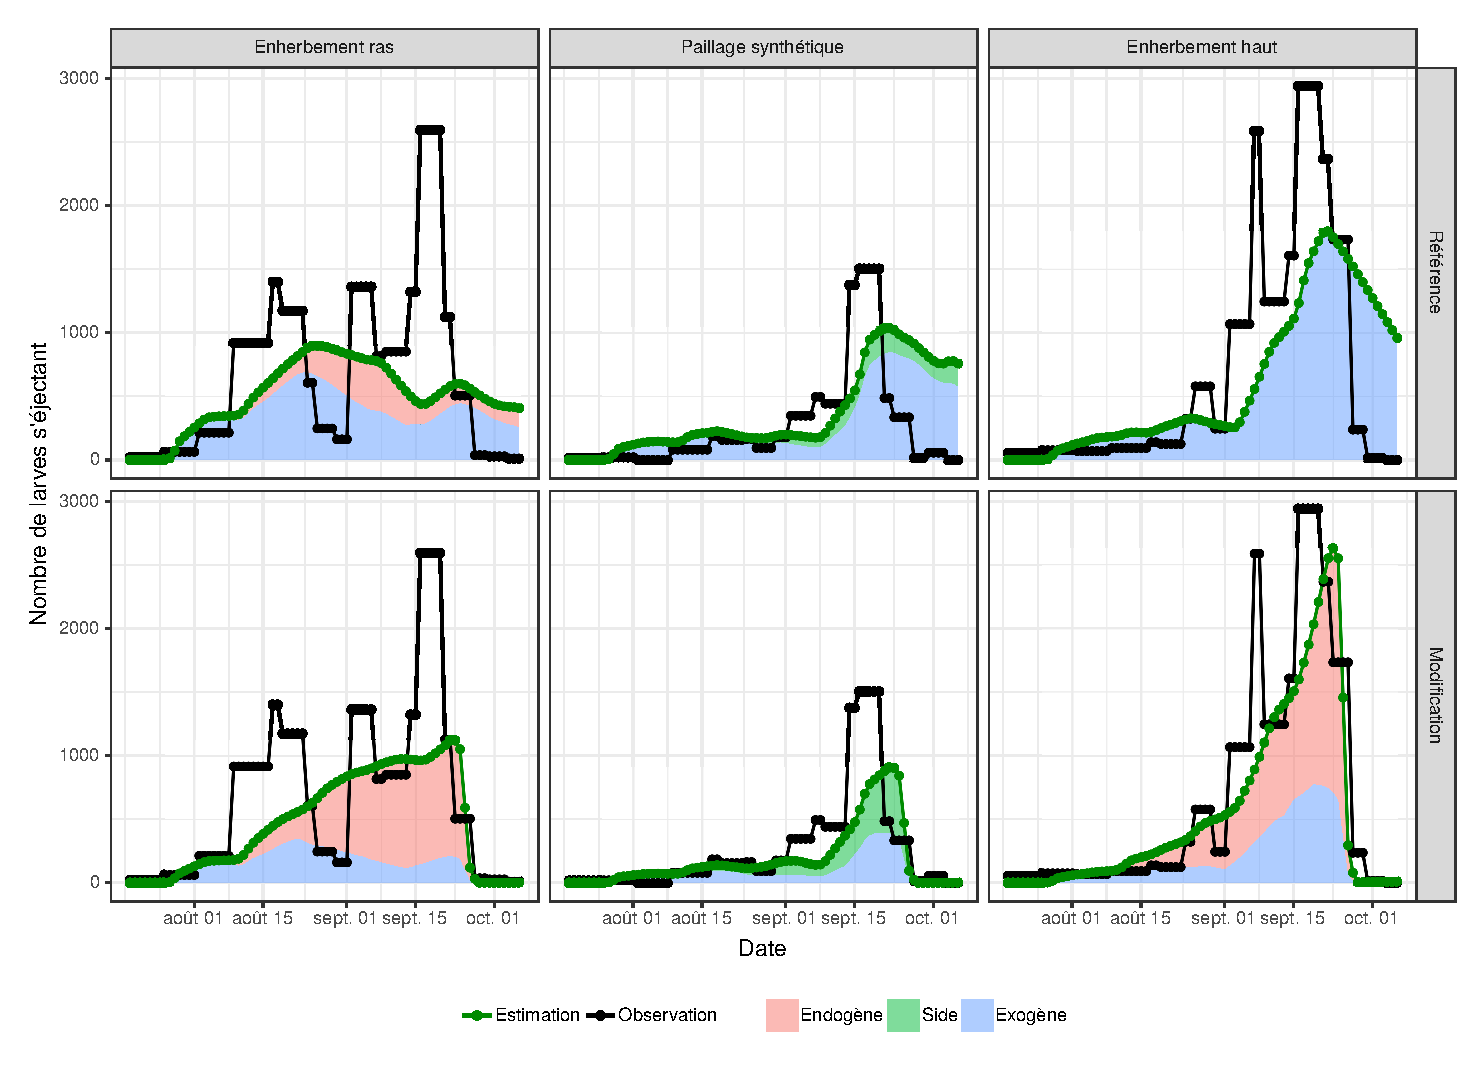
\epsfig{file = plots/proc_end.eps, scale = 0.65}
\caption{Comparaison référence / modification 6.}
\label{fig:end}
\end{figure}







\end{document}

